\documentclass{beamer}

% Copyright 2010 Drow Ltd.
% 
% In principle, this file can be redistributed and/or modified under
% the terms of the GNU Public License, version 2.
% 
% However, this file is supposed to be a template to be modified
% for your own needs. For this reason, if you use this file as a
% template and not specifically distribute it as part of a another
% package/program, I grant the extra permission to freely copy and
% modify this file as you see fit and even to delete this copyright
% notice. 
\mode<presentation>
{
  \usetheme[titleline=true,
  alternativetitlepage=true,
  titlepagelogo=images/Java_logo]{Torino}
  \usecolortheme{nouvelle}
  \beamertemplatenavigationsymbolsempty
}

\usepackage{times}
\usepackage[utf8]{inputenc}
\usepackage[english,bulgarian]{babel}
\usepackage[T2A]{fontenc}

\usepackage{listings}
\lstset{language=Java,
  captionpos=b,
  tabsize=4,
  keywordstyle=\color{blue},
  commentstyle=\color{gray},
  stringstyle=\color{green},
  numbers=left,
  breaklines=true,
  showstringspaces=false,
  basicstyle=\ttfamily,
  emph={label},
  frame=shadowbox, 
  rulesepcolor=\color{blue},
  columns=fixed}

\title{Интерфейси и вътрешни класове}

\author{инж. Божидар ~Бацов}

\institute{Drow Ltd.}

\date{23.11.2010}

\subject{Talks}
% This is only inserted into the PDF information catalog. Can be left
% out. 

\begin{document}

\begin{frame}
  \titlepage
\end{frame}

\begin{frame}{Съдържание}
  \transdissolve
  \tableofcontents[pausesections]
\end{frame}

\section{Интерфейси}

\subsection{Що е интерфейс?}
\begin{frame}{Интерфейс}
  \transdissolve
  \begin{itemize}
  \item
    Наборът от методи, които един клас предлага \pause
  \item
    Езикова конструкция, която съдържа контракт(набор
    от задължения) \pause
  \item Класовете могат да изпълнят контракта(да имплементират
    интерфейса) \pause
  \item Обикновено съдържа само методи \pause
  \item Методите са с ниво на достъп \textbf{public} и са \textbf{абстрактни}
  \end{itemize}
\end{frame}

\subsection{Дефиниция на интерфейс}
\begin{frame}[fragile]
  \frametitle{Дефиниция на интерфейс}
  \transdissolve
\begin{lstlisting}
interface SomeInterface {
  Type field1; // bad style
  Type field2;
  ...
  Type method1();
  Type method2();
}
\end{lstlisting}
\end{frame}

\subsection{Имплементиране на интерфейс}
\begin{frame}[fragile]
  \frametitle{Имплементиране на интерфейс}
  \transdissolve
\begin{lstlisting}
class SomeClass implements SomeInterface {
  ...  
  @Override
  public Type method1() {...}
  @Override
  public Type method2() {...}
}
\end{lstlisting}
\end{frame}

\subsection{Особености на интерфейсите}
\begin{frame}{Особености на интерфейсите}
  \transdissolve
  \begin{itemize}
  \item Всички методи в тях са абстрактни \pause
  \item Един клас може да имплементира повече от един интерфейс \pause
  \item Интерфейсът \textbf{НЕ Е} клас - не може създавате обекти от
    интерфейс \pause
  \item Могат да бъдат декларирани променливи от интерфейсен тип \pause
  \item Работят с instanceof оператора \pause
  \item Не е желателно да имат полета \pause
  \item Абстрактен клас може да имплементира интерфейс напълно или
    частично
  \end{itemize}
\end{frame}

\begin{frame}{Особености на интерфейсите}
  \transdissolve
  \begin{itemize}
  \item Не могат да съдържат instance полета \pause
  \item Не могат да съдържа статични методи \pause
  \item Всички полета в един интерфейс са на практика константи(public
    static final) \pause
  \item Един интерфейс може да разшири(наследи) друг \pause
  \item Интерфейси без методи се използват като маркери(tags)
  \end{itemize}
\end{frame}

\subsection{Интерфейси от стандартната библиотека}
\begin{frame}[fragile]
\frametitle{Сравняване на обекти с интерфейса Comparable}
\transdissolve
\begin{lstlisting}
public interface Comparable<T> {
  int compareTo(T other);
}
\end{lstlisting}
\begin{itemize}
  \item Използва се за сравняване на обекти с естествена подредба
  \item Генеричен интерфейс от Java 5
\end{itemize}
\end{frame}

\begin{frame}[fragile]
  \frametitle{Comparable - пример}
  \transdissolve
\begin{lstlisting}
class Employee implements Comparable<Employee> {
  private double salary;

  ...  

  public int compareTo(Employee other) {
    if (salary < other.salary) return -1;
    if (salary > other.salary) return 1;
    return 0;
  }
}  
\end{lstlisting}
\end{frame}

\begin{frame}{Клониране обекти}
  \transdissolve
  \begin{itemize}
  \item метода clone() на класа Object \pause
  \item интерфейсът Cloneable() - интерфейс маркер \pause
  \item плитко клониране \pause
  \item дълбоко клониране \pause
  \item имплементиране на clone()
  \end{itemize}
\end{frame}

\begin{frame}{Клониране - диаграма}
  \transdissolve
  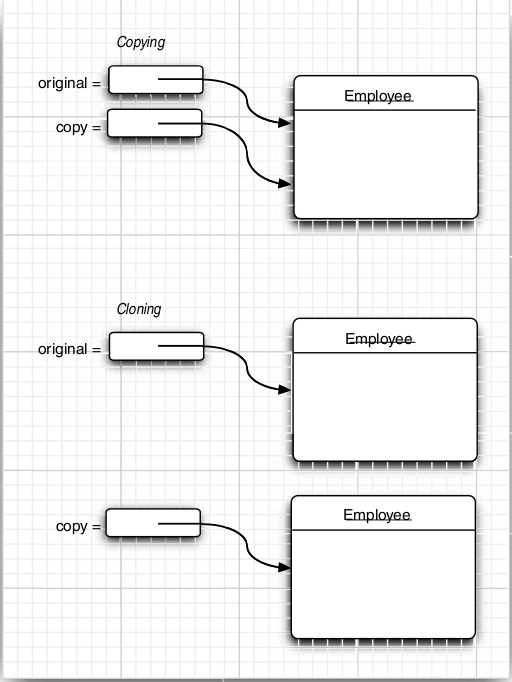
\includegraphics[width=160px,height=160px]{images/cloning.png}
\end{frame}

\begin{frame}{Плитко копиране - диаграма}
  \transdissolve
  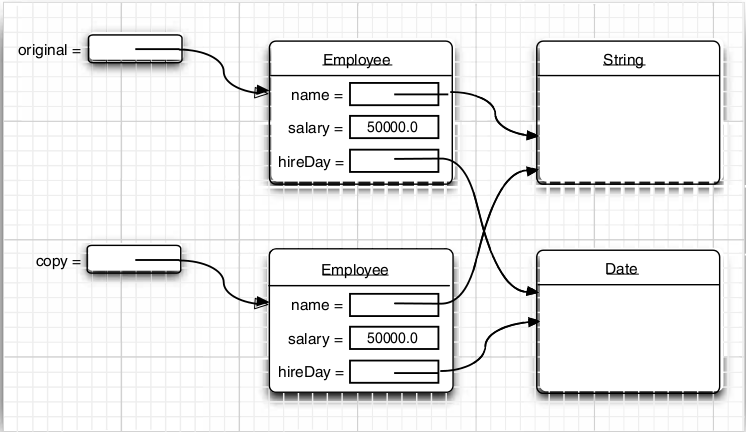
\includegraphics[width=320px,height=160px]{images/shallow-copy.png}
\end{frame}

\begin{frame}[fragile]
  \frametitle{Плитко клониране - пример}
  \transdissolve
\begin{lstlisting}
class Employee implements Cloneable {
  // raise visibility level to public, change return type
  public Employee clone() throws CloneNotSupportedException {
    return (Employee) super.clone();
  }
  . . .
}
\end{lstlisting}
\end{frame}

\begin{frame}[fragile]
  \frametitle{Дълбоко клониране - пример}
  \transdissolve
\begin{lstlisting}
class Employee implements Cloneable
{
  . . .
  public Employee clone() throws CloneNotSupportedException
  {
    // call Object.clone()
    Employee cloned = (Employee) super.clone();
    // clone mutable fields
    cloned.hireDay = (Date) hireDay.clone()
    return cloned;
  }
}  
\end{lstlisting}
\end{frame}

\subsection{Обработка на събития}
\begin{frame}{Обработка на събития}
  \transdissolve
  \begin{itemize}
  \item Събитие \pause
    \begin{itemize}
      \item натиснат бутон \pause
      \item изтекъл таймер \pause
    \end{itemize}
  \item Callback
    \begin{itemize}
      \item код, който се изпълнява в резултат от настъпването на
        дадено събитие \pause
    \end{itemize}
  \item Реализация на callback механизъм с интерфейси
  \end{itemize}
\end{frame}

\begin{frame}[fragile]
  \frametitle{Пример}
  \transdissolve
\begin{lstlisting}[basicstyle=\tiny]
public class TimerTest {
  public static void main(String[] args) {
    ActionListener listener = new TimePrinter();
    // construct a timer that calls the listener
    // once every 10 seconds
    Timer t = new Timer(10000, listener);
    t.start();
    JOptionPane.showMessageDialog(null, "Quit program?");
    System.exit(0);
  }
}

class TimePrinter implements ActionListener {
  public void actionPerformed(ActionEvent event) {
    Date now = new Date();
    System.out.println("At the tone, the time is " + now);
    Toolkit.getDefaultToolkit().beep();
  }
}
\end{lstlisting}
\end{frame}

\section{Вътрешни класове}
\subsection{Какво са вътрешните класове?}
\begin{frame}{Вътрешни класове}
  \transdissolve
  \begin{itemize}
  \item Влагане да дефиницията на един клас в друг \pause
  \item Реализирани са на ниво компилатор \pause
  \item Позволяват достъп до членовете на класа, в който са вложени \pause
  \item Видове \pause
    \begin{itemize}
      \item стандартни \pause
      \item локални  \pause
      \item анонимни \pause
      \item статични \pause
    \end{itemize}
  \end{itemize}
\end{frame}

\subsection{Стандартни вътрешни класове}
\begin{frame}{Стандартни вътрешни класове}
  \transdissolve
  \begin{itemize}
  \item Дефинирани са в друг клас на нивото на полетата и методите му \pause
  \item Имат достъп до полетата и методите на външния клас \pause
  \item Имат скрита референция към външния клас \pause
  \item Всяка инстанция от външния клас носи дефиницията на вътрешния
  \end{itemize}
\end{frame}

\begin{frame}[fragile]
  \frametitle{Пример}
  \transdissolve
\begin{lstlisting}[basicstyle=\tiny]
class TalkingClock {
  private int interval;
  private boolean beep;

  public TalkingClock(int interval, boolean beep) {
    this.interval = interval;
    this.beep = beep;
  }
  
  public void start() {
    ActionListener listener = new TimePrinter();
    Timer t = new Timer(interval, listener);
    t.start();
  
  }
  // inner class
  private class TimePrinter implements ActionListener {
    public void actionPerformed(ActionEvent event) {
      Date now = new Date();
      System.out.println("At the tone, the time is " + now);
      if (beep) Toolkit.getDefaultToolkit().beep();
    }
  }
}
\end{lstlisting}
\end{frame}


\begin{frame}{Вътрешен клас}
  \transdissolve
  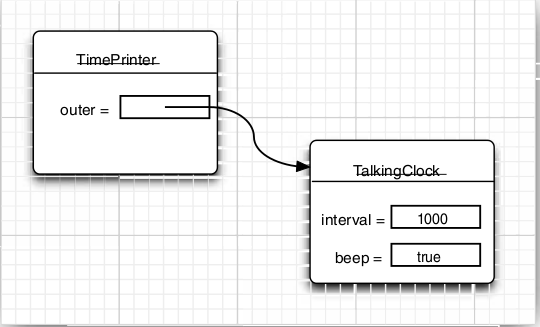
\includegraphics[width=320px,height=160px]{images/inner-class.png}
\end{frame}


\subsection{Локални вътрешни класове}
\begin{frame}{Локални вътрешни класове}
  \transdissolve
  \begin{itemize}
  \item Дефинирани са в тялото на метод на външния клас \pause
  \item Имат достъп до локалните променливи в метода \pause
    \begin{itemize}
      \item но само до тези маркирани като final \pause
    \end{itemize}
  \item Не са видими извън метода, в който са дефинирани
  \end{itemize}
\end{frame}

\begin{frame}[fragile]
  \frametitle{Пример}
  \transdissolve
\begin{lstlisting}[basicstyle=\small]
public void start() {
  class TimePrinter implements ActionListener {
    public void actionPerformed(ActionEvent event) {
      Date now = new Date();
      System.out.println("At the tone, the time is " + now);
      if (beep) 
        Toolkit.getDefaultToolkit().beep();
    }
  }
  ActionListener listener = new TimePrinter();
  Timer t = new Timer(interval, listener);
  t.start();
}  
\end{lstlisting}
\end{frame}

\subsection{Анонимни вътрешни класове}
\begin{frame}{Анонимни вътрешни класове}
  \transdissolve
  \begin{itemize}
  \item Разновидност на локалните класове \pause
  \item Създава се обект от клас дефиниран след оператора за
    присвояване \pause
  \item Обикновено анонимните класове имплементират някой интерфейс
    \pause
  \item Не могат да дефинират собствени конструктори
  \end{itemize}
\end{frame}

\begin{frame}[fragile]
  \frametitle{Пример}
  \transdissolve
\begin{lstlisting}[basicstyle=\small]
public void start(int interval, final boolean beep) {
  ActionListener listener = new ActionListener() {
    public void actionPerformed(ActionEvent event) {
      Date now = new Date();
      System.out.println("At the tone, the time is " + now);
      if (beep) 
        Toolkit.getDefaultToolkit().beep();
    }
  };
  Timer t = new Timer(interval, listener);
  t.start();
} 
\end{lstlisting}
\end{frame}

\subsection{Статични вътрешни класове}
\begin{frame}{Статични вътрешни класове}
  \transdissolve
  \begin{itemize}
  \item Еквивалентни на стандартните, но без референция към външния
    клас  \pause
  \item Служат като допълнително пространство на имената
  \end{itemize}
\end{frame}

\begin{frame}[fragile]
  \frametitle{Пример}
  \transdissolve
\begin{lstlisting}
class Outer {
  ...

  public static class Inner {
    ...
  }
}  
\end{lstlisting}
\end{frame}

\section*{Заключение}
\begin{frame}{Заключение}
  \transdissolve
  % Keep the summary *very short*.
  \begin{itemize}
  \item
    Интерфейсите са проста алтернатива на множественото наследяване.
  \item
    Вътрешните класове ви дават възможност да изразите по-прецизно
    връзките между класовете ви.
  \end{itemize}
  
  % The following outlook is optional.
  \vskip0pt plus.5fill
  \begin{itemize}
  \item
    Следващият път:
    \begin{itemize}
    \item
      Разработка на графични потребителски интерфейси със Swing
    \end{itemize}
  \end{itemize}
\end{frame}

\begin{frame}{Въпроси}
  \transdissolve
  \begin{center}
    \LARGEТук е момента да зададете вашите въпроси! :-)
  \end{center}
\end{frame}

\begin{frame}{Край}
  \transdissolve
  \begin{center}
    \LARGEБлагодаря Ви за вниманието!
  \end{center}
\end{frame}

\end{document}

%%% Local Variables: 
%%% mode: latex
%%% TeX-master: t
%%% End: 
